\clearpage
\subsection{BLDC-Betrieb}
Der Brushless-DC Betrieb (BLDC) ist dadurch gekennzeichnet, dass zwei Stränge gegensätzlich und der dritte überhaupt nicht bestromt werden. Dadurch ergeben sich für den Stromraumzeiger nur 6 mögliche diskrete Richtungen im Abstand von jeweils \SI{60}{\degree} zueinander (vgl. links in Abbildung \ref{fig:bldc_schema}). Für die Bestimmung des Umschaltzeitpunktes ist kein teurer Lagesensor mehr nötig - es sind z.B. simple Hallelemente vollkommen ausreichend. Dieser Vorteil wird dadurch erkauft, dass aufgrund der doch recht groben Diskretisierung der möglichen Stromraumzeiger im Großteil der Rotorpositionen keine ideale Momentenausbeute möglich ist. Damit sinkt ausgehend vom maximalen Moment bei idealer Lage eines Stromraumzeigers (dem Fluss $90\degree$ voreilend) mit steigendem Lagewinkel $\gamma_m$ (ist hier gleich dem Winkel zwischen Flussverkettungsraumzeiger und $\alpha$-Achse) das verfügbare Moment $m_R$ kosinusförmig, bis es beim Eintritt des Flussraumzeigers in den neuen Sektor wieder in der gleichen Form ansteigt und dann abermals das Maximum erreicht, wenn der Fluss dem aktuellen Sektor-Stromraumzeiger um genau $90\degree$ nacheilt (vgl. rechts in Abbildung \ref{fig:bldc_schema}).  

\begin{figure}[h!]
    \centering
    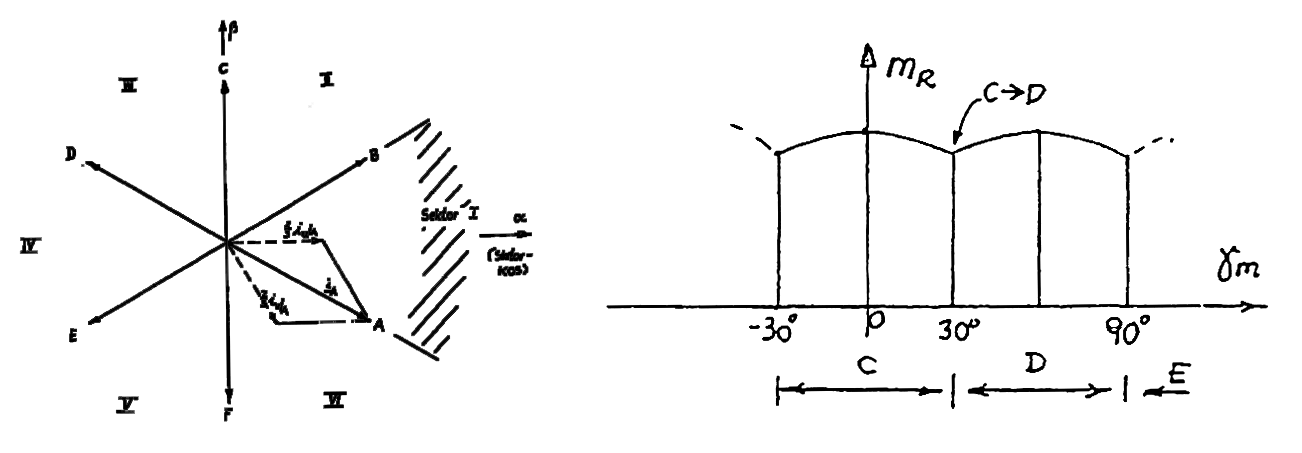
\includegraphics[scale=0.55]{2/BLDC.png}
    \caption{Diskrete Raumzeiger mit Sektoren im statorfesten KOS (links) und Momentenverlauf in Abhängigkeit der Rotorposition (rechts).}
    \label{fig:bldc_schema}
\end{figure}

%Finde ich ein wenig ungenau formuliert - bitte nicht köpfen, lg Thomas %Da der Stromraumzeiger für \SI{60}{\degree} Blöcke konstant bleibt, entsteht kein konstantes Drehmoment mehr, sondern ein cosinusförmiges laut folgender Gleichung
%\begin{equation*}
%    m_R(\tau) = - Im \left[ \underline{i}^*_s \underline{\Psi}_S\right] = - Im \left[ \underline{i}^*_s \big( \underline{\Psi}_M \big) \right] = \underline{\Psi}_M \cdot i_{s,d} = \underline{\Psi}_M  i_{s} \cdot sin(\gamma_m)
%\end{equation*}

\noindent Im Zuge eines erneuten Drehzahlsprunges wurden die Ströme in dieser Betriebsart gemessen. Diese sind als Stromortskurve in Abbildung \ref{fig:stromortskurve_bldc} dargestellt und zeigen die erwarteten diskreten Stromraumzeiger. Die abweichenden Stromraumzeiger, die mitten in den Sektoren zum Liegen kommen, sind auf ... ?? .. zurückzuführen.

\input{\currfiledir stromortskurve.tex}
\input{\currfiledir sprung_bldc.tex}

\noindent Weiters ist der entsprechende Zeitverlauf der Messgrößen dieses Versuches in Abbildung \ref{fig:sprung_bldc} dargestellt.
